\documentclass[a4paper,12pt]{article}
\usepackage{graphicx}
\usepackage[left=30mm, right=30mm, top=30mm, bottom=35mm]{geometry}
\usepackage{amsmath}
\usepackage{siunitx}
\usepackage{fancyhdr}
\usepackage{url}
\pagestyle{fancy}
%-------------------------------------------------------------------------------
\lhead{\textbf{Spring 2019}}
\rhead{\textbf{CE394M Advanced Analysis in Geotechnical Engineering}}
\cfoot{\thepage}
%-------------------------------------------------------------------------------

\begin{document}
\begin{centering}
	\textbf{
		Assignment 3: FEM Structural analysis\\
		Assigned: 14th February 2019\\
		Due: 1st March 2019\\
	}
\end{centering}

\vspace{1em}
 
\begin{enumerate}

	\item Consider the following structural system consisting of a three-noded triangle and a cable
	element (i.e. two-noded one-dimensional element). The triangle element is fixed at the (local) nodes 1 and 3 and its stiffness matrix for the unconstrained degrees of freedom at node 2 is
	
		\begin{equation*}
			\mathbf{K} = 10^9 %
			\begin{bmatrix}
				1.97	& 0 \\ 
				0 & 0.66 \\
			\end{bmatrix}
			%
			\begin{matrix}
				u_{x2}^e\\ 
				u_{y2}^e \\
			\end{matrix}	
		\end{equation*}
		
		For the cable, the product of the Young’s modulus and cross-sectional area is $EA = 1.0\cdot 10^9$.
		Further, the system is loaded with a nodal force of $f_{y2} = -10000$.
		
		\begin{figure}[!h]
			\centering
			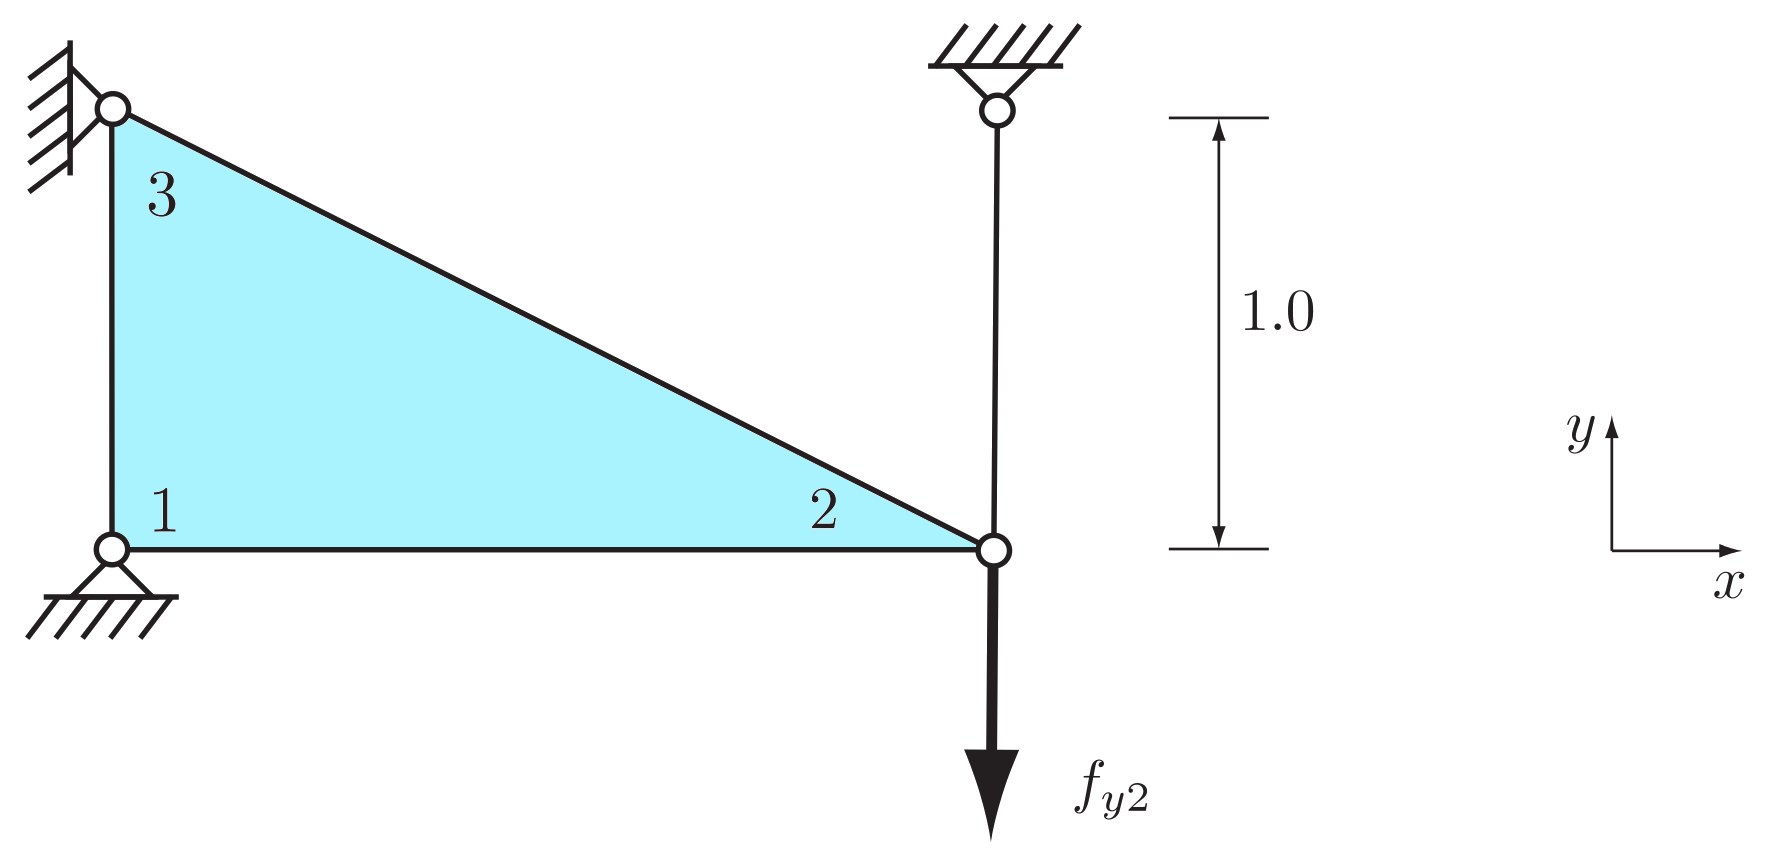
\includegraphics[width=0.5\textwidth]{figs/2d-truss.png}
		\end{figure}
	
		\begin{itemize}
			\item Determine the displacements $u_{x2}$ and $u_{y2}$ of node 2.
			\item Determine the force in the cable.
		\end{itemize}
	
	
	\item Using the Jupyter notebook for elastic-bar-linear.ipynb (available on Canvas) compute and plot the displacement profiles for the following loading conditions. Discretize the cantilever beam using linear elements.
	
		\begin{itemize}
			\item A uniformly distributed load of 1.
			\item A uniformly varying load with 1 at the fixed end, and 0 at the free end.
			\item A sinusoidal load described as $f(x) = \sin(x^2)$
		\end{itemize}
	
		\begin{enumerate}
			\item Calculate the error in the displacement, using the FE solution with 100 elements as the reference solution.
			\item Use at least 5 different discretizations and plot how the error changes with the number of elements.
			\item Based on the errors computed above, determine the number of linear elements required to perform a FE analysis for each of the three loading conditions shown above.
		\end{enumerate}
	
\end{enumerate}

\end{document}

